\chapter{Preguntas tecnicas Java y Spring}
\section{Diferencias entre Spring y Spring Boot}
Es un proyecto de Spring.Se añade un servidor de aplicaciones embebido,autoconfiguraciones
y elimina el trabajo con XML.Es decir configuraciones en XML.
\section{Que es un Bean}
Es una pieza de software que representa un objeto dentro de spring .Son manejados por el contenedor de
spring.Tiene un ciclo de vida.Son reusables.
\section{Que es el ambito de un bean}
Define el ciclo de vida y visibilidad del bean en el contexto.Se define con la anotacion @Scope.\\
Singleton :Por defecto y rara vez sera necesario usar otro diferente.El bean va a tener la misma
instancia durante todo el aplicativo.\\
Prototype:Es una copia de una instancia.\\
Request: Crea una nueva instancia por cada peticion HTTP ,solo en una aplicacion web se puede utilizar.\\
Session: Crea una instancia por cada sesion HTTP.\\
Application\\
Websocket\\
\section{Que son los starters y cual es su objetivo}
Es una utilidad que facilita la creacion y configuracion de aplicaciones.\\
Agregan dependencias necesarias para un objetivo y parametros de configuracion.Ejemplo:
spring-boot-starter-web\\
spring-boot-starter-data-jpa
\section{Cuales son las principales verbos/metodos HTTP y como se pueden implementar con Spring Boot}
Se pueden implementar con Spring Boot.\\
GET @GetMapping : Para obtener informacion.\\
POST @PostMapping : Utilizado para enviar informacion.\\
PUT @PutMapping : Reemplaza el contenido del recurso con el nuevo.\\
DELETE @DeleteMapping : Borra la informacion del recurso especificado.\\
PATCH @PatchMapping : Aplica modificaciones parciales al recurso especificado.
\section{Que diferencia existe entre JPA e Hibernate}
Java Persistance API define una especificacion o interfaces para el manejo de persistencias.\\
Hibernate es una impplementacion particular de JPA.Y es usado ppor defecto en Spring Boot.
JPA es una especificacion e hibernate es una implementacion.
\section{Que es Spring Initializer}
Esuna plataforma online para generar un proyecto base de Spring Boot.Se puede usar por la web
directamente o desde los principales IDES como STS o Intellij.
\section{Que diferencias existen entre @Repository @Service
	@Component @Controller}
No existen diferencias funcionales,solo semanticas.Son anotaciones para marcar clases en Spring y que se creen benas a ppartir de ellas .Ejemplo.:Las clases tipo servicio(@Component,@Service).
\section{Explique la anotacion @RestController}
Facilita la creacion de API REST usando spring MVC.
Combina @Controller+@RequestBody.Permite serializar cualquier respuesta de un controlador
Spring MVC directamente a json o XML..
\section{Que es Spring AOP}
AOP significa programacion orientada a aspectos.
Permite crear aspectosen nuestras aplicaciones para ser usados de forma transversal
Ejemplo.: Crear una anotacion que permite auditar la realizacion  de determinadas acciones.
\section{La anotacion @Profile que funcion tiene y porque es importante}
@Profile permite usar beans determinados en dependencia del perfil activo en una aplicacion Spring Boot.\\
Los perfiles permiten instancias de forma particular una aplicacion en dependencia de un escenario por ejemplo: dev,qa,prod.
\section{Que hace la anotacion @SpringBootApplication internamente}
Anotaci\'on principal de spring boot,ubicada por defecto en la clase principal de un proyecto de spring boot.
Combina alas anotaciones de :\\
 @Configuration\\
 @EnableAutoConfiguration\\
 @ComponentScan\\
Permite inicilizar todo lo necesario para que nuestra aplicacion SpringBoot pueda iniciar a trabajar correctamente.
\section{Que patrones estan presentes en Spring/SpringBoot agregue un ejemplo}
Creacional:Singleton.Ejemplo:Al crear un bean anotando una clase con @Service y @Scope por defecto usamos singleton.\\
Estructural:Proxy.Ejemplo.:Usado por @Transactional para los sistemas de persistencia.\\
Comportamiento:Cache Template. 
\section{Para que se usa @TransacTional}
En BD una operacion es transactional si mantiene el estado en un sistema consistente.\\
@Transactional permiteejecutar operaciones en spring en forma de todo o nada.Si algo sale mal durante la ejecucion de una operacion @Transactional el sistema se deja en su estado inicial.
\section{Que es la inyeccion de dependencias}
DI es un patron para separar responsabilidades evitando que una clase sea responsable de instanciar objetos de otra.Promueve el bajo acoplamiento.\\
Al arrancar Spring se crean los objetos (beans) y luego se inyectan donde son necesarios usando @Autowired.
\section{Cuales son las formas de inyecccion de dependencias que existen en Spring y cual es el mas adecuado}
Inyeccion por atributo.\\
Inyeccion por setter.\\
Inyeccion por constructor;Facilita el testeo de la aplicacion de una manera mas sencilla.
\section{Para que se usa @Value y que lenguaje usa la anotacion para su funcion}
@Value permite leer configuraciones y colocarlas en la propiedad anotada.Usa lenguaje SpEL.Ejemplo.:
\begin{lstlisting}
@Value("${value.from.file}")
\end{lstlisting}
\section{Cual es el puerto por defecto de una aplicacion Spring Boot y como podemos cambiarlo}
Por defecto es el puerto 8080.Se cambia en la propiedad server.port del fichero de configuracion.
\section{Que es Spring Actuator}
Libreria que proporciona herramientas de monitoreo y administracion para un API REST.\\
Habilita varios endpoints para ser usados .Ejemplo:/beans\\/health\\/shutdown.\\
Permite ser extendido
\section{Que es Spring Cloud}
Spring Cloud es un proyecto basado en Spring Boot .\\
Implementa soluciones production-ready para el desarrollo de microservicios.\\
Algunos componentes son: Spring	Cloud Config.\\
Spring Cloud Gateway.\\
Esta influenciado por NetflixOSS.
\section{Spring IoC Conteiner}
Es el contenedor priincipal de Spring.Utiliza las inyecciones de independencias para administrar
el ciclo de vida de todos los objetos que Spring va a gestionar.
\section{Que es un Autowired}
Es la tecnica o forma de como hacer las inyecciones automaticamente de las instancias de los beans.\\
Con la anotacion @Autowired.
\section{Como indicas que bean utilizar}
Mediante la anotacion @Qualifine me permite indicar el nombre exacto del bean que necesito.Tambien con
@Primary.
\section{Como se gestionan las transacciones en Spring}
Se trabaja mediante el uso de @Transactional.
\section{Se puede trabajar Spring solo con java}
Tambi\'en se puede trabajar con Kotlin y Groovy.
\section{Cuales son los archivos de configuraci\'on de Spring Boot}
application.property (yml/properties).\\
Bootstrap.yml.
\section{Cuales son los estereotipos de Spring y que funciones cumplen}
@Repository : Contextualizar la clase para acceso a B.D..\\
@Service : Contextualizar la clase para l\'ogica de negocios.\\
@Controller : Contextualizar la clase para que sea un controlador.\\
@Component : Contextualizar la clase para que sea un utilitario.\\
Cuando se estereotipa una clase se puede hacer una inyeccion de dependencias de una instancia
de esa clase.
\section{Las aplicaciones que SpringApplication resume}
@SpringBootConfiguration.\\
@EnableAutoConfiguration.\\
@ComponentScan.
\section{Que contenedores embebeidos puede tener Spring Boot}
Tomcat y Jetty.
\section{Como ejecutas en consola el codigo de Spring}
Se debe implementar la interface comand Nai Runner.
\section{Como lees el archivo properties}
Mediante @Value para extraer la informaci\'on mediante una llave
\section{Establecer entornos de QA,DEV,PROD}
Se usa properties para cada entorno y se reconoce mediante sufijos .\\
Application-dev.properties\\
Application-test.properties\\
Application-prod.properties\\
\section{Spring Boot es compatible con proyectos antiguos de Spring}
Si es compatible usando la anotacion @importVisors
\section{Que anotacion usas para obtener el json y enviarlo en objeto en java}
@RequestBody.
\section{Como se gestiona el tema de la internalizaci\'on o 18n}
El local resolver maneja concepto de bundle.Se puede cambiar el tema del idioma 
a las respuestas que Spring ofrece.
\section{Spring Security forma parte de Spring Framework}
No forma parte , es un proyecto independiente como cloud,data,batch.
\section{Defina la arquitectura de microservicios}
Es un enfoque para desarrollar una aplicaci\'on como un conjunto de peque\~nos servicios.\\
Cada uno de los cuales se ejecuta en su propio proceso.\\
Se comunican con mecanismos ligeros.\\
Estos servicios se basan en el negocio y se pueden implementar de forma independiente.\\
Existe un minimo de gesti\'on de centralizada de estos servicios.\\
Pueden escribirse en diferentes lenguajes de programaci\'on y utilizar diferentes tecnologias de almacenamiento de datos.
\section{Ventajas de arquitectura de microservicios}
Perrmite asignar equipos especificos peque\~nos y manejables.\\
Permite implementar pruebas de forma mas atomicas.\\
Permite implementar pruebas de integraci\'on sectorrizadas.\\
Es posible usar las tecnologias mas adecuadas en cada microservicio.Por ejemplo : Para busqueda de
clientes y productos,podemos incorporar un Elastic Search para busqueda de texto completo.\\
Facilita desagregar el despliegue de ciertos micrroserrvicios en diversos nodos y con multiples instancias a
demanda (Escalamiento horizntal).
\section{Implementar los retos para la arquitectura de microservicios}
Lograr un dise\~no adecuado.\\
Gesti\'on de la infraestructurra.\\
Correcta gesti\'on de la transaccionalidad y la consistencia de los datos.\\
Gestion del entorno distrribuido y asumir las 8 falacias de la computaci\'on distribuida son un elemento a tene en cuenta
en la implementaci\'on.\\
Necesidad de la implementaci\'n de la cultura DevOps.
\section{En la arquitectura de microservicios como se puede resolver el problema de los parametros
 de configuraci\'on de los microservicios y sus instancias}
Patr\'on de configuraci\'on centralizada.Spring Cloud Config.
\begin{figure}[H]
	\centering
	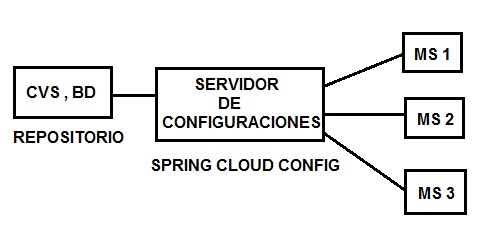
\includegraphics[scale=0.7]{images/fig_1_1.jpg}
	\caption{Spring Cloud Config}
\end{figure}
\section{En una arquitectura de microservicios son comunes las llamadas servicio-servicio que mecanismos
	puede implementar para evitar posibles fallos}
Debemos conocer las falacias de la computaci\'n distribuida.\\
Dar una soluci\'on con reintentos.\\
Dar una soluci\'on con Circuit Breaker.
 \section{Porque Java Developer}
 Es un lenguaje altamente demandado por las industrrias y diversos sectorres.Java esta consolidado y abierto a un abanico de posibilidades.
\section{Tenemos una semana de atraso, como afrontarias esta situaci\'on de estres}
Tratar de evaluar la situacion actual, dar solucion a lo prioritario y despues resolver los otros items de acuerdo a los tiempos y apoyo que brinden el equipo en conjunto. 
\section{Porque java es independiente}
Es gracias a la maquina virrtual que java es multiplataforma y se puede usar en cualquier sistema operativo.
\section{En que situaciones utilizarias los tipos de dato wrappe} 
Los wrapper pueden tener valores nulos.
\section{Los conceptos claves de POO}
Encapsulamiento : Prrotege el codigo de las demas varriables prrivadas.Getter Setter.\\
Herencia : Una clase puede extenderrse a otra clase\\
Polimorfismo : Tiene muchas formas.Un objeto puede referrirse a la subclase o superclase segun el tipo de referrencia.\\
Abstraccion: Se selecciona los datos esenciales de un objeto para ser mostrados y oculta otros elementos menos rrelevantes.
\section{Una interface puede heredar o implementar una interface}
Una iinterface solo puede heredar otra interface.Las clases son las que implementan las interfaces.
\section{Cuando usarrias una clase abstracta de una interface}
Una clase puede implementar n interfaces (Herencia multiple) .Una herencia tradicional se puede usar una clase abstracta.
\section{Cuando se usaria una list o un set}
Una lista permite valores repetidos . Un set (Hash set) no pemite valores duplicados solo uno nomas se tomara en cuenta. 
\section{Cuantos metodos abstractos o no implementados puede tener una interface funcional}
Una interfaz funcional solo puede tener un metodo abstracto.Para que mas adelante a partir de esa interface se pueda generar 
una expresion lamda.
\section{Cual es la difeencia entre List y ArayList}
List es la interface y ArrayList es la implementacion de esa interface.
\section{Interrfaces funcionales que ofrece java}
Las mas comunes son el predicate (Test) , consumer (Void) , suplayer (Retorna un objeto).
\section{Cuando usarrias Runnnable y thread en una clase}
Runnable es una interface y thread es una clase.\\
Cuando la clase tenga extend se usaria la interface Runnable.\\
Si el proceso es asincrono y trabaja de la forma tradicional se puede heredar a thread.\\
Si se quisiera implementar varias interfaces y aparte heredar a otras clases seria mejor usar runnable.
Asi pudiendo sobreescribir sus metodos.
\section{Que es la sincronizacion en java}
Se debe esperar para que un proceso termine.Para poderr pasar al siguiente.Protegiendo la zona critica (asincrono).\\
Asincrono : Thread,runnable,webflux.
\section{Comprueba usted su codigo}
Aplico TDD y trabajo con librerias Junit,Mockito.Tecnicas de definicion de escenarios.
\section{Como ejecutas javascript desde java}
Con Nashoin y jjs.
\section{De un conjunto de elementos,como eliminar los elementos duplicados}
Con el API stream con filter y disting.\\
Transformamos la lista a Set (Uso la clase colector).
\section{Comenta sobrre el esquema de licencia Java}
Java 17 : Es gratis LTS.Hasta un año despues dela prroxima libreria.\\
Java 11 : En prroduccion es de pago\\
Java 8 : Empieza ser de pago.\\
Nota : Amazon Coretto es gratis.
\section{Cambios de java 8 a 11/17}
Eliminacion de modulos Java EE.\\
Sintaxis de varriables locales para parametros CORBA en lambdas (@NotNull).\\
Un cliente HTTP (java.net.http).\\
Ejecucion desde archivo de codigo fuente unico.\\
Soporte unicode IO.\\
Nuevos metodos para nuestros Strings : isBlank(),lines(),strrip(),repeat(int).\\
Lectura y escritura de string en archivos(readString(path),writeString().\\
Acceso a clases interrnas mediante metodos que usan reflexion.\\
Eliminacion de codigo no deseable,deprrecables u obsoletos.
\section{Programacion funcional}
Los lenguajes de programacion funcional son aquellos lenguajes donde las variables no tienen estado.
\section{Streams}
Los streams simplemente ejecutan el flujo de trabajo para el primer elemento o el elemento que cumpla
la condicion dada.El flujo termina.Esto permite mejorar el rendimiento ya que no es necesario recorrer
 la lista completa.\\
 Son envoltorios de condiciones de datos que nos permite operar con estas colecciones y hacer que el procesamiento
 masivo de datos sea rapido y facil de leer.
\section{Lambda}
Son expresiones anonimas , es decir funciones que no necesitan una clase. (parametros) -> { cuerpo-lambda} .\\
Tipos de lambda : Consumidores,proveedores,funciones(op. unitarios,binarios).Predicados.\\
Consumidores : Acepta un solo valor y no devuelve valor alguno.\\
Proveedores : Expresiones que no tienen parametros,sin embargo devuelven un resultado.\\
Funciones : Aceptan un argumento y devuelven un valor como resultado(Cuyos tipos no tienen que ser iguales).\\
Predicados : Se trata de expresiones que aceptan un parametro y devuelven un valor logico. 
\section{Java optional}
Hace referencia a una variable  que puede tener un valor asignado o que puede contener un valor
 null.Metodos isPresent,get().
\section{Patrones de Arquitectura}
Patron de capas : \\
Patron cliente-servidor : \\
Patron maestro esclavo : \\
Patron bus : \\
Patron MVC : \\
Patron pizarra : 
\section{Como activa un perfil}
En application.prroperrties se agrega : spring.prrofiles.active=dev.\\
La siguiente popiedad en la VM : DSping.profiles.active=dev.
\section{SPEL}
Es un lenguaje de expresiones que permite realizar operaciones sobre la informacion en
tiempo de ejecucion.
\section{AOP}
Agrega comportamioento a codigo existente sin necesidad de modificarlo.\\
Creacion de aspecto,se define un bean de sprring y se anota con @Aspect.Se define
el metodo que se ejecutara con el advice.@Before,@AfterReturning,@After.\\
Nota : Si se tiene multiples advices es posible definir el orden con @Order.
\section{Peticion HTTP}
Metodo HTTP,URI,version de protocolo utilizado,heades,body.
\section{Respuesta HTTP}
Version del protocolo,status code,headers,body.Status Http:\\
1xx : Informacional.\\
2xx : Peticion exitosa.\\
3xx : Redirecciones.\\
4xx : Error del lado del cliente.\\
5xx : Error del lado del serrvidor. 
\section{Soporte para REST}
Se debe incluir el modulo Spring MVC.Mediante la dependencia : \\
spring-boot-stater-web
\section{Configuracion de metricas}
Es posible crear metricas propias para analizar el funcionamiento de mi app.Dependencia : \\
micrometer-registry-prometheus\\
Consulta de metricas : /actuator/prometheus
\section{Dependencias para usar Swagger}
springfox-swagger2\\
spring-swagger-ui\\
Para configurar swagger se debe configurar un docket.\\
Para acceder a la documentacion por defecto:\\
http://localhost:8080/swagger-ui.html
\section{Configuracion de Cache}
Se agrega la dependencia spring-boot-starter-cache.\\
La anotacion @EnableCaching.\\
Una vez configurado se debe agregar los objetos al cache ,para esto @Cacheable("Codes").\\
Es posible revocar valores de un cache a traves de @CacheEvict.
\section{Concurrent MapCacheManager}
Concurrent MapCacheManage el cache se realiza en la maquina que esta ejecutando la app.
\section{Integracion con REDIS}
Para hacer la integracion con redis,se agrega la dependencia redisson.\\
Agregamos el bean de redison al contexto.\\
Modificamos el CacheManager,para indicar a spring que use redis.\\
Nota : Los objetos que se escriban en el cache deben implementar la interfaz serializable.
\section{Cuales son los chicos malos.seguridad}
El sitio web debe protegerse debido a imitadores,mejoradores y espias.\\
Imitadores:Doble identificacion MFA de este modo se combina el saber algo(Password) con el tener algo(certificado).\\
Mejoradores: Permisos suficientes para acceder a un recurso.Esto se consigue mediante la configuracion de ROLES.\\
ROL es un grupo de usuarios que tiene acceso a un conjunto de recursos especificos.Un usuario puede tener multiples roles.\\
Espias: Confidencialidad.El cifrado de datos es un metodo comun para asegurar la confidencialidad.
\section{Cambiar password en spring segurity}
spring-boot-stater-securrity.Para cambiar el password por defecto de application.properties:\\
spring.security.user.name\\
spring.security.user.password
\section{Spring Segurity autentificacion contra una B.D.}
Se debe implementar la interfaz UserDetails.No se valida el password , solo se obtiene de la base de datos.
\section{Formas de proteger apliaciones Spring Boot}
Usar HTTPS en produccion.\\
Usar snyk para verificar tus dependencias.\\
Actualizar la ultima version.\\
Habilitar proteccion CSRF.\\
Use estrategias de seguridad de contenido para evitar ataques XSS.
\section{Security Context Holder}
Es una clase que permite acceder a la informacion tanto del usuario como del rol.\\
Nota: Los roles serran modificados por spRing agregando el prefijo ROLE.Ejemplo : ROLE\_ADMIN
\section{Global Security Config}
Clase que permite asegurar a nivel de metodo en esta clase se agrega la notacion @EnableBlobalMethodSecurrity.
\section{@Secured}
En spring nos permite definir la lista de roles permitidos al ejecutar un metodo.
\section{@RolesAllowed}
Es equivalente a @Secured,la diferencia es que la primera no es propia de spring.
\section{@PreAuthorize @PostAuthorize}
@PreAuthoize: Hace una evaluacion antes de ejecutar el metodo, dependiendo del resultado de la evaluacion decide si ejecutalo o no.\\
@PostAuthorize: Permite realizar una evaluacion despues de ejecutar el metodo,dependiendo del resultado de la evaluacion decide devolver o no el valor.Meta anotaciones es posible crear metaanotaciones.\\
Nota: Para combinar el uso de las anotaciones de seguridad.\\Ejemplo: @IsUserOrAdmin tendra el mismo efecto que usar 
@PreAuthorize y @PostAuthorize.
\section{Status HTTP 403}
El error indica que el usuario tiene una autentificacion exitosa, pero fallo al realizar la autorizacion.
\section{S.O.L.I.D.}
S Principio de responsabilidad unica : Un obejeto deberria tener una unica razon para cambiar. \\
O Principio de abierto o cerrado : Las entidades de software deben estar abiertas para su extension, pero cerrados para su modificacion.\\
L Principio de sustitucion de Liskov : Los objetos de un programa deberia ser reemplazables por instancias de sus subtipos
sin alterar el correcto funcionamiento del programa. \\
I Principio de segregacion de interfaz : Muchas interfaces cliente especificas son mejores que una interfaz de proposito general.\\
D Principio de inversion de dependencias : Se debe depender de abstracciones,no depender de implementaciones.
\section{Artifactory}
Artifactory es un Repositorio de Maven. En el se pueden desplegar las dependencias\\
 que necesiten los proyectos en maven para su ciclo de vida. Otra de las principales\\
  funciones de artifactory es hacer de proxy cache de un repositorio propio con otros existentes.\\
  Facilidad de instalación.\\
  Facilidad de configuración.\\
  Soporte para múltiples repositorios locales.
\section{Sonar Cube}
Se puede ver la calidad del codigo.Analiza,hace test,auditoria.No se recomienda usar la BD embebida.
\section{Jenkins,jmeter}
Jenkins ayuda en la automatización de parte del proceso de desarrollo de software mediante integración continua y facilita ciertos aspectos de la entrega continua. Admite herramientas de control de versiones como CVS, Subversion, Git, Mercurial y puede ejecutar proyectos basados en Apache Ant y Apache Maven.
\section{Streams que mas has usado.Map}
Agrupacion de elementos sobrelos que podemos especificar operaciones.\\
Map es para convertir .\\
filter es para filtrar.\\
sorted es para ordenar.\\
reduce opera sobre los elementos de un stream.
\section{Diferencias entre Rest y SOAP}
Rest es una arquitectura en cambio SOAP es un protocolo que necesita un contrato(WDSL).\\
Rest es mas sencillo de usar.\\
El codigo es declarativo.\\
Mejor gestion de la complejidad.\\
Integracion de la API funcional.\\
Uso potencial del paralelismo.
\section{Que es una interfaz funcional}
Interface con solo un metodo abstract,puede tener metodos default.\\
Con @FunctionalInterface, el compilador valida que es una funcional interface.
\section{SCRUM}
Los roles en SCRUM son :\\
 Product Owner:Es la representacion del cliente dentro del equipo de trabajo.responsable de expresar
 claramente la necesida del cliente dentro del Product Backlog.Define el Product Backlog\\
Scrum Master :Responsable de aseguarar que el SCRUM es entendido y realizado por el equipo.
El equipo debe trabajar ajustandose a la teoria,practica y reglas de SCRUM\\
El Team Developer :Responsables de dar cumplimiento a los SPRINT.\\
Reunion Sprint Planning Meeting.
Resultado de esta reunion se tiene el Sprint Backlog,son conjuntos de requisitos que se deben cumplir en una o 4 semanas.(Este tiempo es el SPRINT)\\
En el SPRINT intervienen el scrum master y team developer .\\
Los Daily son los seguimientos diarios no deben durar mas de 15 min.\\
Al final de un SPRINT se hace una reunion llamada sprint review(ScrumMaster,Team developer y product owner),se revisa la entrega o el producto invremental.\\
 Despuees de entregar el producto se hace una reunion Sprint Retrospective.Mejoras o problemas\\
 \section{Patrones de microservicios}
 Patron Saga: Es una secuencia de transacciones locales donde cada transacci\'on  actualiza informaci\'on 
 dentro de un servicio.
 \section{Patrones de diseno software}
 builder :  un patr\'on de construcci\'on para construir objetos. A veces, los objetos que creamos pueden ser complejos, estar formados por varios subobjetos.\\
 Observer: Este patr\'on es una dependencia de uno a muchos entre objetos, de modo que cuando un objeto cambia de estado, se notifica a todos sus dependientes.\\
 Singleto : se utiliza para limitar la creaci\'on de una clase a un solo objeto. Esto es beneficioso cuando se necesita un objeto (y solo uno) para coordinar acciones en todo el sistema. \\
 Adapter :Esto permite que las clases incompatibles trabajen juntas al convertir la interfaz de una clase en otra. Piense en ello como una especie de traductor: cuando dos jefes de estado que no hablan un idioma com\'un se encuentran, generalmente un intérprete se sienta entre los dos y traduce la conversaci\'on, lo que permite la comunicaci\'on.\\
 Proxy :  un proxy es un contenedor o un objeto de agente que el cliente est\'a llamando para acceder al objeto de
  servicio.
 \section{OWASP}
 OWASP Security Framework, que es una aplicaci\'on web que explica los principios de codificaci\'on segura en m\'ultiples lenguajes de programaci\'on y tiene como objetivo ayudar a los desarrolladores a crear aplicaciones seguras por dise\~no.
 \section{Tipos de arquitectura de Software}
  Arquitectura  MVC, la programaci\'on por capas, peer-to-peer, orientada a servicios (SOA), cliente-servidor.
  \section{Arquitectura Limpia}
  Independientes del framework.\\
  Testables.\\
  Independientes de la UI\\
  Independientes de la base de datos.\\
  Independiente de agentes externos\\
  Más tolerantes al cambio\\.
  Reutilizables.\\
  Mantenibles.
  \section{ Arquitectura  Hexagonal}
    La intenci\'on de la Arquitectura Hexagonal no es otra que permitir que una aplicaci\'on sea usada de la 
    misma forma por usuarios, programas, pruebas automatizadas o scripts, y sea desarrollada y probada de
     forma aislada de sus eventuales dispositivos y bases de datos en tiempo de ejecuci\'on.\\
      Tambi\'en conocida como arquitectura de puertos y adaptadores, tiene como principal motivaci\'on separar
       nuestra aplicaci\'on en distintas capas o regiones con su propia responsabilidad. De esta manera consigue
        desacoplar capas de nuestra aplicaci\'on permitiendo que evolucionen de manera aislada. Adem\'as, tener 
        el sistema separado por responsabilidades nos facilitar\'a la reutilizaci\'on.
\section{RxJava}
\section{AKS,funcions,cosmoDB}
\section{Circuit Breaker}
\section{Programacion reactiva como lo has usado,dependencias}

\section{Pruebas de test unitario,mockito}
\section{Webflux}
\section{Bitbacket}
\section{Spring Cloud Config server}
\section{Spring Security}
\section{MongoDB}
\section{Monitoreo Kibana,prometheus,grafena,new relic}
\section{git privacy}
\section{Jenkins, Prometheus, Grafana, Logstash, Kibana, Fluentd}
\section{ORM}